\chapter{Fundamentação Teórica}

\section{Considerações Iniciais}

Podem-se estabelecer algumas premissas para guiar o projeto de filtros:
\begin{itemize}
\item{\textbf{Linearidade e Invariância no Tempo}}: Para filtros analógicos, essa premissa é bastante clara visto que componentes eletrônicos reais não podem ter seus valores e características modificados facilmente. Dessa forma, o sistema inteiro é tratado como LTI (\textit{Linear Time-Invariant}), facilitando a implementação do circuito e permitindo o emprego da transformada de Laplace para análise no domínio da frequência. 

Similarmente, para filtros digitais, uma das principais ferramentas de análise é a transformada Z, a qual também tem um sistema LTI como premissa.\footnote{Existem filtros digitais cujo comportamento é não-linear - por exemplo, o filtro de Kalman - porém, eles não serão abordados neste trabalho.} 

Desta forma, a linearidade permite o uso de ferramentas matemáticas convenientes e poderosas (transformadas Z e Laplace, convolução, superposição etc...) as quais resultam na simplificação do processo de projeto \cite{oppenheim}.

\item{\textbf{Causalidade}:} para aplicação em tempo real, um filtro deverá ser causal, isto é, depender apenas da entrada atual e das entradas anteriores. Isso requer que, para uma função de transferência qualquer dada por $Y(s) = \dfrac{N(s)}{D(s)}$, o grau de $N(s)$ seja menor que o grau de $D(s)$, e que ambos graus sejam finitos; isto equivale a dizer que, para qualquer $t < 0$, $y(t) = 0$ (ou, para sistemas discretos, $y_n = 0$ para $n < 0$) \cite{oppenheim}.

\item{\textbf{Estabilidade}:} visto que os circuitos empregados em filtros ativos possuem \textit{feedback}, o critério BIBO (\textit{bounded in, bounded out}), o qual garante que para uma entrada finita, teremos uma saída finita (isto é, existe um valor $B > 0$ tal que $|y(t)| \leq B$ para todo $t$ em sistemas analógicos ou $|y_n| \leq B$ para todo $n$ em sistemas digitais), torna-se um critério importante \cite{oppenheim}; caso contrário, podem ocorrer problemas de estabilidade com o sinal filtrado. Em uma implementação prática, teremos saturação ou oscilação na saída se esse critério for violado. 

Em filtros digitais existem considerações sobre o tamanho máximo das variáveis (uma variável de $n$ bits\footnote{Em geral, $n$ = 8, 16, 32 ou 64 bits, os tamanhos mais comuns de variáveis na linguagem C} pode armazenar um valor máximo de $2^n - 1$ sem sinal ou uma faixa de valores de $-2^{n-1}$ a $2^{n-1}-1$ com sinal): é necessário implementar lógica para tratar \textit{overflows} e \textit{underflows} \cite{smith_dsp}. 

\item{\textbf{Implementação}:} para filtros analógicos, torna-se necessário definir valores de componentes disponíveis no mercado, suas características (por exemplo, a largura de banda e a \textit{slew rate} do amplificador operacional) e suas respectivas tolerâncias de forma a obter um circuito que na prática forneça a função de transferência especificada. \cite{jung} Em altas frequências ou quando sinais de amplitude muito baixa estão envolvidos, também surgem questões ligadas ao ruído dos dispositivos empregados.

Já para filtros digitais é necessária a escolha de um dispositivo computacional (microprocessador, microcontrolador, DSP, FPGA)\footnote{A partir daqui, quando for mencionado \textit{CPU}, entenda-se qualquer um desses dispositivos.} e de conversores analógico-digital e digital-analógico que atendam às especificações necessárias e que sejam capazes de executar a quantidade necessária de operações no intervalo entre uma amostra e outra.

Para um sinal cuja largura de banda seja $f_{bw}$, o critério de Nyquist faz com que seja necessária uma frequência de amostragem $f_s$ de no mínimo $2 f_{bw}$ \cite{haykin}: na prática ela será muito maior, para capturar o conteúdo do sinal até a harmônica desejada. Assim, o período que a CPU terá para realizar todas as operações (leitura do conversor A/D, cálculo, acesso à memória RAM e saída para o conversor D/A) deverá ser de no máximo $1/{f_s}$.

A maioria das CPUs modernas possui conversores analógico-digital (A/D) e digital-analógico (D/A) integrados; se estes forem usados, é necessário considerar as limitações inerentes (por exemplo, número de bits e velocidade de amostragem) a esses; caso demonstrem-se insuficientes, é necessário interfaceamento de conversores externos - o que aumenta o tempo de conversão, pois se faz necessária a comunicação com os dispositivos para a leitura e a escrita de dados.

Considerado que uma das principais aplicações de CPUs é no processamento de sinais digitais, muitos fabricantes incluem instruções de multiplicação e acumulação (\textit{multiply and accumulate}), realizadas por \textit{hardware} dedicado dentro da CPU, que realizam a operação $y \leftarrow y + (a * b)$, na qual $y$ é um acumulador e $a$ e $b$ são variáveis, em um número mínimo de ciclos de \textit{clock} \cite{dspic}. 

Surgem, também, problemas de precisão numérica que podem afetar os resultados, principalmente para altas frequências de amostragem e na operação em ponto flutuante. Assim, torna-se necessário estruturar o algoritmo para tentar minimizar esses impactos ou, se possível - considerado que isso incorre em uma perda de precisão - utilizar ponto fixo. \cite{smith_dsp}

\end{itemize}

\section{Tipos de filtros}

Podem ser descritos cinco principais tipos de filtro, cujas respostas em frequência estão visualizadas na tabela \ref{table:filter_generic_freq_response}:

\begin{itemize}
\item{\textbf{Filtro passa-baixa} (\textit{low-pass}):} um filtro deste tipo irá rejeitar todas as frequências $f > f_c$, onde $f_c$ é a frequência de corte estabelecida.
\item{\textbf{Filtro passa-alta} (\textit{high-pass}):} este filtro irá se comportar de forma oposta ao filtro passa-baixa, rejeitando todas as frequências $f < f_c$.
\item{\textbf{Filtro passa-faixa} (\textit{band-pass}):} é a junção dos dois tipos de filtro anteriores; para uma frequência de centro $f_c$ e uma largura de banda (\textit{bandwidth}) $B$, teremos que o filtro deixará sinais cuja frequência esteja no intervalo dado por $f_c - B$ e $f_C + B$.
\item{\textbf{Filtro rejeita-faixa} (\textit{band-stop}):} apresenta comportamento oposto ao filtro passa-faixa, rejeitando as frequências que estejam entre $f_L = f_c - B$ e $f_H = f_C + B$. Para $B$ muito pequeno (ou seja, um filtro que rejeita uma faixa muito específica de frequências), é chamado de filtro \textit{notch}.
\item{\textbf{Filtro passa-todas} (\textit{all-pass}):} este filtro não modifica a amplitude do sinal (isto é, a resposta em frequência dele é plana), apenas a fase dele.
\end{itemize}


\begin{table}[h]
\centering
\begin{tabular}{ll}
\textbf{a. }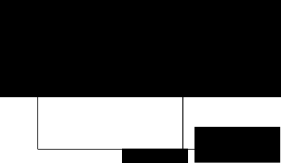
\includegraphics[scale=0.7]{images/lowpass_generic} \newline  & \textbf{b.} 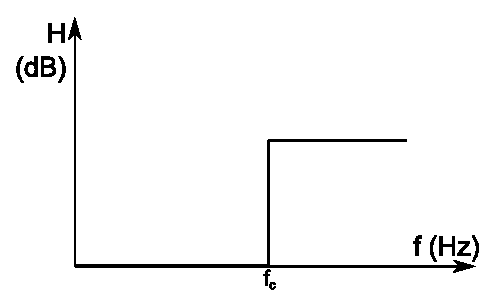
\includegraphics[scale=0.7]{images/highpass_generic}  \\
\textbf{c.} 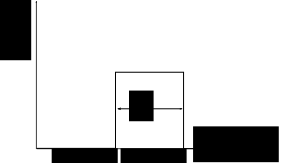
\includegraphics[scale=0.7]{images/bandpass_generic}  & \textbf{d.} 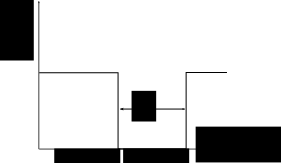
\includegraphics[scale=0.7]{images/bandstop_generic} 
\end{tabular}
\caption{Respostas em frequência genéricas dos filtros descritos.}
\label{table:filter_generic_freq_response}

\end{table}

\section{Filtros Analógicos}
\label{sec:analog_filters}
Os filtros acima descritos são comumente chamados de \textit{brick wall} ou filtro sinc, pois a sua representação no domínio do tempo é dada por funções da família $sinc(x) = \frac{\sin x}{x}$ \cite{haykin}; são ideais e impossíveis de serem implementados na prática, por violarem a premissa de linearidade e invariância no tempo. Dessa forma, torna-se necessária uma função de transferência que consiga aproximar a resposta desejada. Comumente são empregadas cinco diferentes implementações, as quais serão descritas a seguir.

\subsection{Funções de Transferência de Filtros Analógicos}

\subsubsection{Filtro de Butterworth}
A resposta em frequência de um filtro Butterworth passa-baixa, de ordem $n$ e frequência\footnote{As funções de transferência serão expressadas em termos de $\omega = 2 \pi f_0$ pois isso simplifica sua representação} de $-3$ dB $\omega_c = 2 \pi f_c$, para uma frequência $\omega$ é dada por

\begin{equation}
H(j\omega) = \sqrt{\frac{G_0}{1 + {(\dfrac{\omega}{\omega_c}})^{2n}}}
\label{eq:butterworth_tf}
\end{equation}

onde $G_0$ é o ganho em $\omega = 0$. Alternativamente, pode-se afirmar que os polos do filtro de Butterworth de ordem $N$, para $\omega = 1$, estão posicionados no plano complexo conforme a relação 

\begin{equation}
p_k = \omega_0 \frac{\sin{(2k-1)\pi}}{2n} + j \frac{\cos{(2k-1)\pi}}{2n}
\label{eq:butterworth_poles}
\end{equation}

para $k = 1 \dots n$. 

Filtros de Butterworth, como descritos em \cite{butterworth}, são marcados por uma resposta em frequência sem ondulações (\textit{ripple}) na banda de passagem - assim, eles são empregados quando a característica de planicidade é desejável; todavia, sua transição da frequência de passagem (\textit{passband}) para a frequência de corte (\textit{stopband}) é bastante lenta em comparação aos outros filtros. 

% \footnote{\textit{Um filtro elétrico ideal deverá não só rejeitar completamente as frequências indesejadas, mas ter sensitividade uniforme nas frequências desejadas.}}

\newpage

\subsubsection{Filtro Chebyshev, tipo 1}
A resposta em frequência de um filtro Chebyshev tipo 1 passa-baixa com \textit{ripple} $\epsilon$ na banda passante é \cite{sedra_smith}:

\begin{equation}
H_n(\omega) = \dfrac{1}{\sqrt{1+\epsilon^2 T_n^2 (\dfrac{\omega}{\omega_c})}}
\label{eq:cheby1_tf}
\end{equation}

Onde $T_n$ é o polinômio de Chebyshev de ordem $n$, definido pela relação de recorrência $T_{n+1}(x) = 2 x T_{n}(x) - T_{n-1}(x)$ para $T_0(x) = 1$ e $T_1(x) = x$.

O valor de $\epsilon$ para um determinado \textit{ripple} em dB é dado pela relação 

\begin{equation}
\epsilon_{dB} = 20 \log \sqrt{1+\epsilon^2}
\label{eq:cheby_ripple}
\end{equation}

Similarmente, seus polos estão distribuídos no plano complexo em uma elipse, dada pela relação

\begin{equation}
p_k = -\omega_0 \sin\frac{(2k-1)\pi}{2n} \sinh(\frac{1}{n} \sinh^{-1}\frac{1}{\epsilon}) + j\omega_0 \cos\frac{(2k-1)\pi}{2n} \cosh(\frac{1}{n} \sinh^{-1}\frac{1}{\epsilon})
\label{eq:cheby1_poles}
\end{equation}

para $k = 1 \dots n$.

Este filtro é um meio-termo entre o filtro de Butterworth e o filtro elíptico: na figura \ref{fig:compare_freqs} é fácil ver que ele apresenta inclinação intermediária entre a banda de passagem e a banda de parada, não apresentando \textit{ripple} nesta última.

\subsubsection{Filtro Chebyshev, tipo 2}
Filtros Chebyshev tipo 2 - também chamados de \textit{Chebyshev inverso} por alguns autores \cite{zumbalen} - apresentam \textit{ripple} na banda de parada, em contraste ao filtro tipo 1 que apresenta este fenômeno na banda de passagem. A resposta em frequência de um filtro passa-baixa, de ordem $n$ e frequência de $-3$ dB $\omega_c$, para uma frequência $\omega$ é dado por \cite{sedra_smith}:

\begin{equation}
H_n(\omega) = \dfrac{1}{\sqrt{1+\frac{1}{\epsilon^2 T_n^2 (\dfrac{\omega_c}{\omega})}}}
\label{eq:cheby2_tf}
\end{equation}

sendo o parâmetro $\epsilon$ referente à atenuação na banda de parada; para uma atenuação $\gamma$ em dB, ele é dado pela expressão

\begin{equation}
\epsilon = \frac{1}{\sqrt{10^{\gamma/10} - 1}}
\end{equation}.

Seus polos são o inverso dos polos determinados na equação \ref{eq:cheby1_poles}, para o filtro Chebyshev tipo 1. Para este filtro, excepcionalmente, define-se $\omega_c$ como sendo a frequência onde a atenuação especificada é atingida.

\subsubsection{Filtro de Bessel}
A resposta em frequência de um filtro Bessel passa-baixa, de ordem $n$ e frequência de $-3$ dB $\omega_c$, para uma frequência $\omega$ é dada por 

\begin{equation}
H(\omega) = \frac{\theta_n(0)}{\theta_n(\frac{\omega}{\omega_0})}
\label{eq:bessel_tf}
\end{equation}

onde $\theta_n$ é o polinômio de Bessel, determinado pela recorrência $\theta_n(x) = (2n-1)\theta_{n-1}(x) + x^2 \theta_{n-2}(x)$, de ordem $n$.

Os polos de um filtro Bessel de ordem $n$ estão distribuídos no plano complexo em um círculo, espaçados em $\frac{2}{n}$, exceto nos dois polos mais próximos do eixo y, que estarão espaçados em $\frac{1}{n}$. Uma das características mais importantes desse tipo de filtro é sua resposta de fase linear. 

\subsubsection{Filtro Elíptico}
A resposta em frequência de um filtro elíptico\footnote{ou filtro de Cauer, em homenagem a Wilhelm Cauer} passa-baixa, de ordem $n$ e frequência de $-3$ dB $\omega_c$, para uma frequência $\omega$ é dada por

\begin{equation}
H(\omega) = \frac{1}{1 + \epsilon^2 R^2_n (\dfrac{\omega}{\omega_c})}
\label{eq:ell_tf}
\end{equation}

onde $R_n$ é uma função elíptica \footnote{Funções elípticas pertencem a uma classe de funções especiais, que surgiram a partir de problemas de cálculo envolvendo elipses.}. Em geral, devido ao seu cálculo mais complexo - e que não será abordado aqui devido à exigência das funções especiais, estando disponível em \cite{paarmann} - são usados valores tabelados.

A principal vantagem deste filtro é ter a transição da \textit{passband} para a \textit{stopband} mais rápida possível, ao custo de introduzir um \textit{ripple} em ambas as bandas.

As respostas dos filtros são exemplificadas na figura \ref{fig:compare_freqs}. O gráfico dos polos das funções de transferência é apresentado na figura \ref{fig:compare_poles}. Do gráfico podemos concluir que, quanto mais próximos os polos estiverem da origem, maior o \textit{ripple} e mais rápida é a transição. 

\begin{figure}[H]
\centering
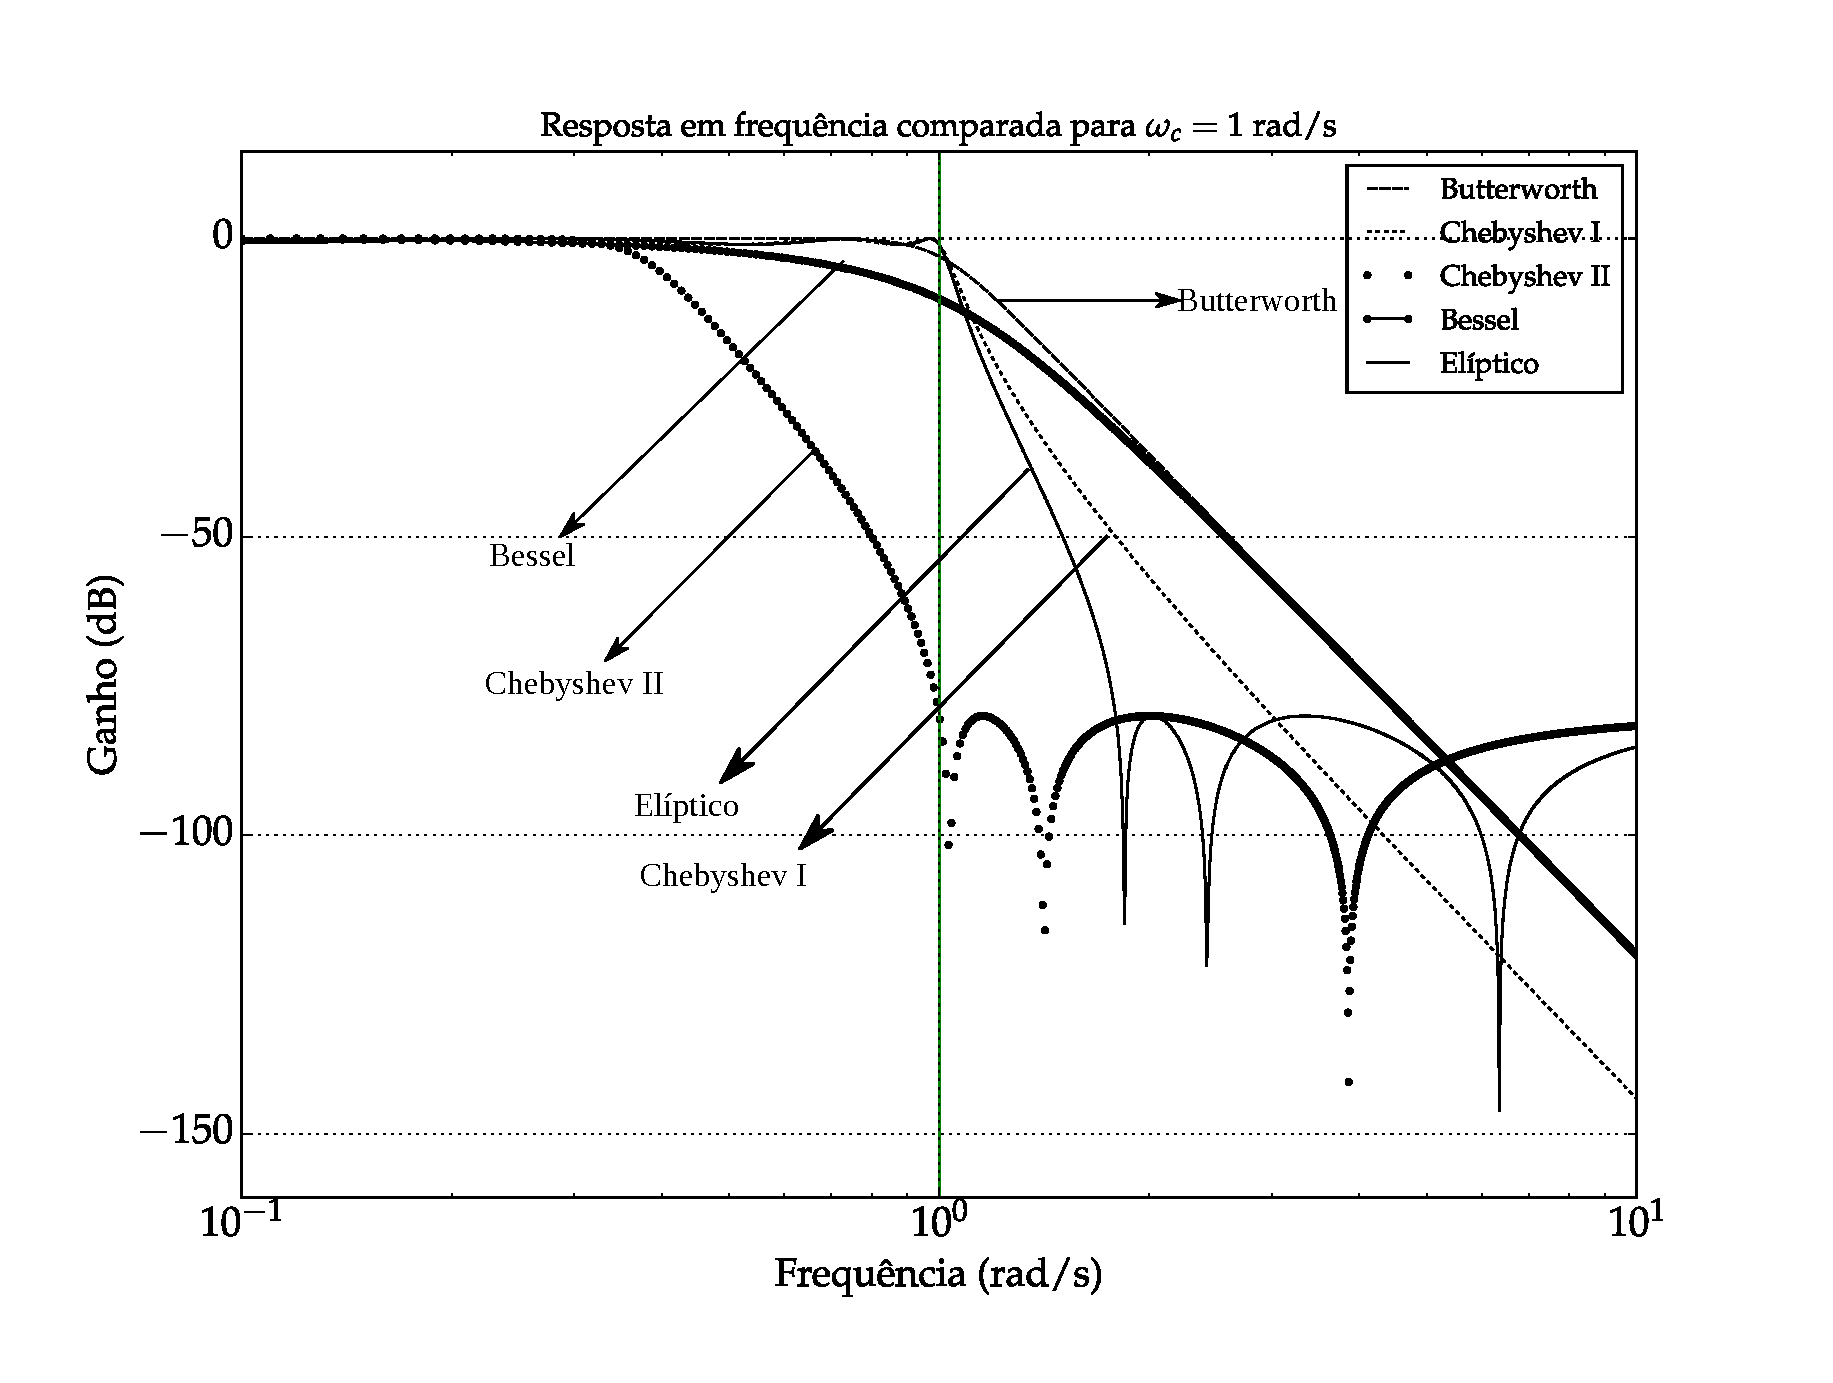
\includegraphics[scale=0.58]{images/plots/compare_frequencies}
\caption{Comparação das respostas em frequência para filtros \textit{low-pass} com $\omega_c$ = 1 rad/s. Todos os filtros têm ordem $N = 6$.}
\label{fig:compare_freqs}
\end{figure}

\begin{figure}[H]
\centering
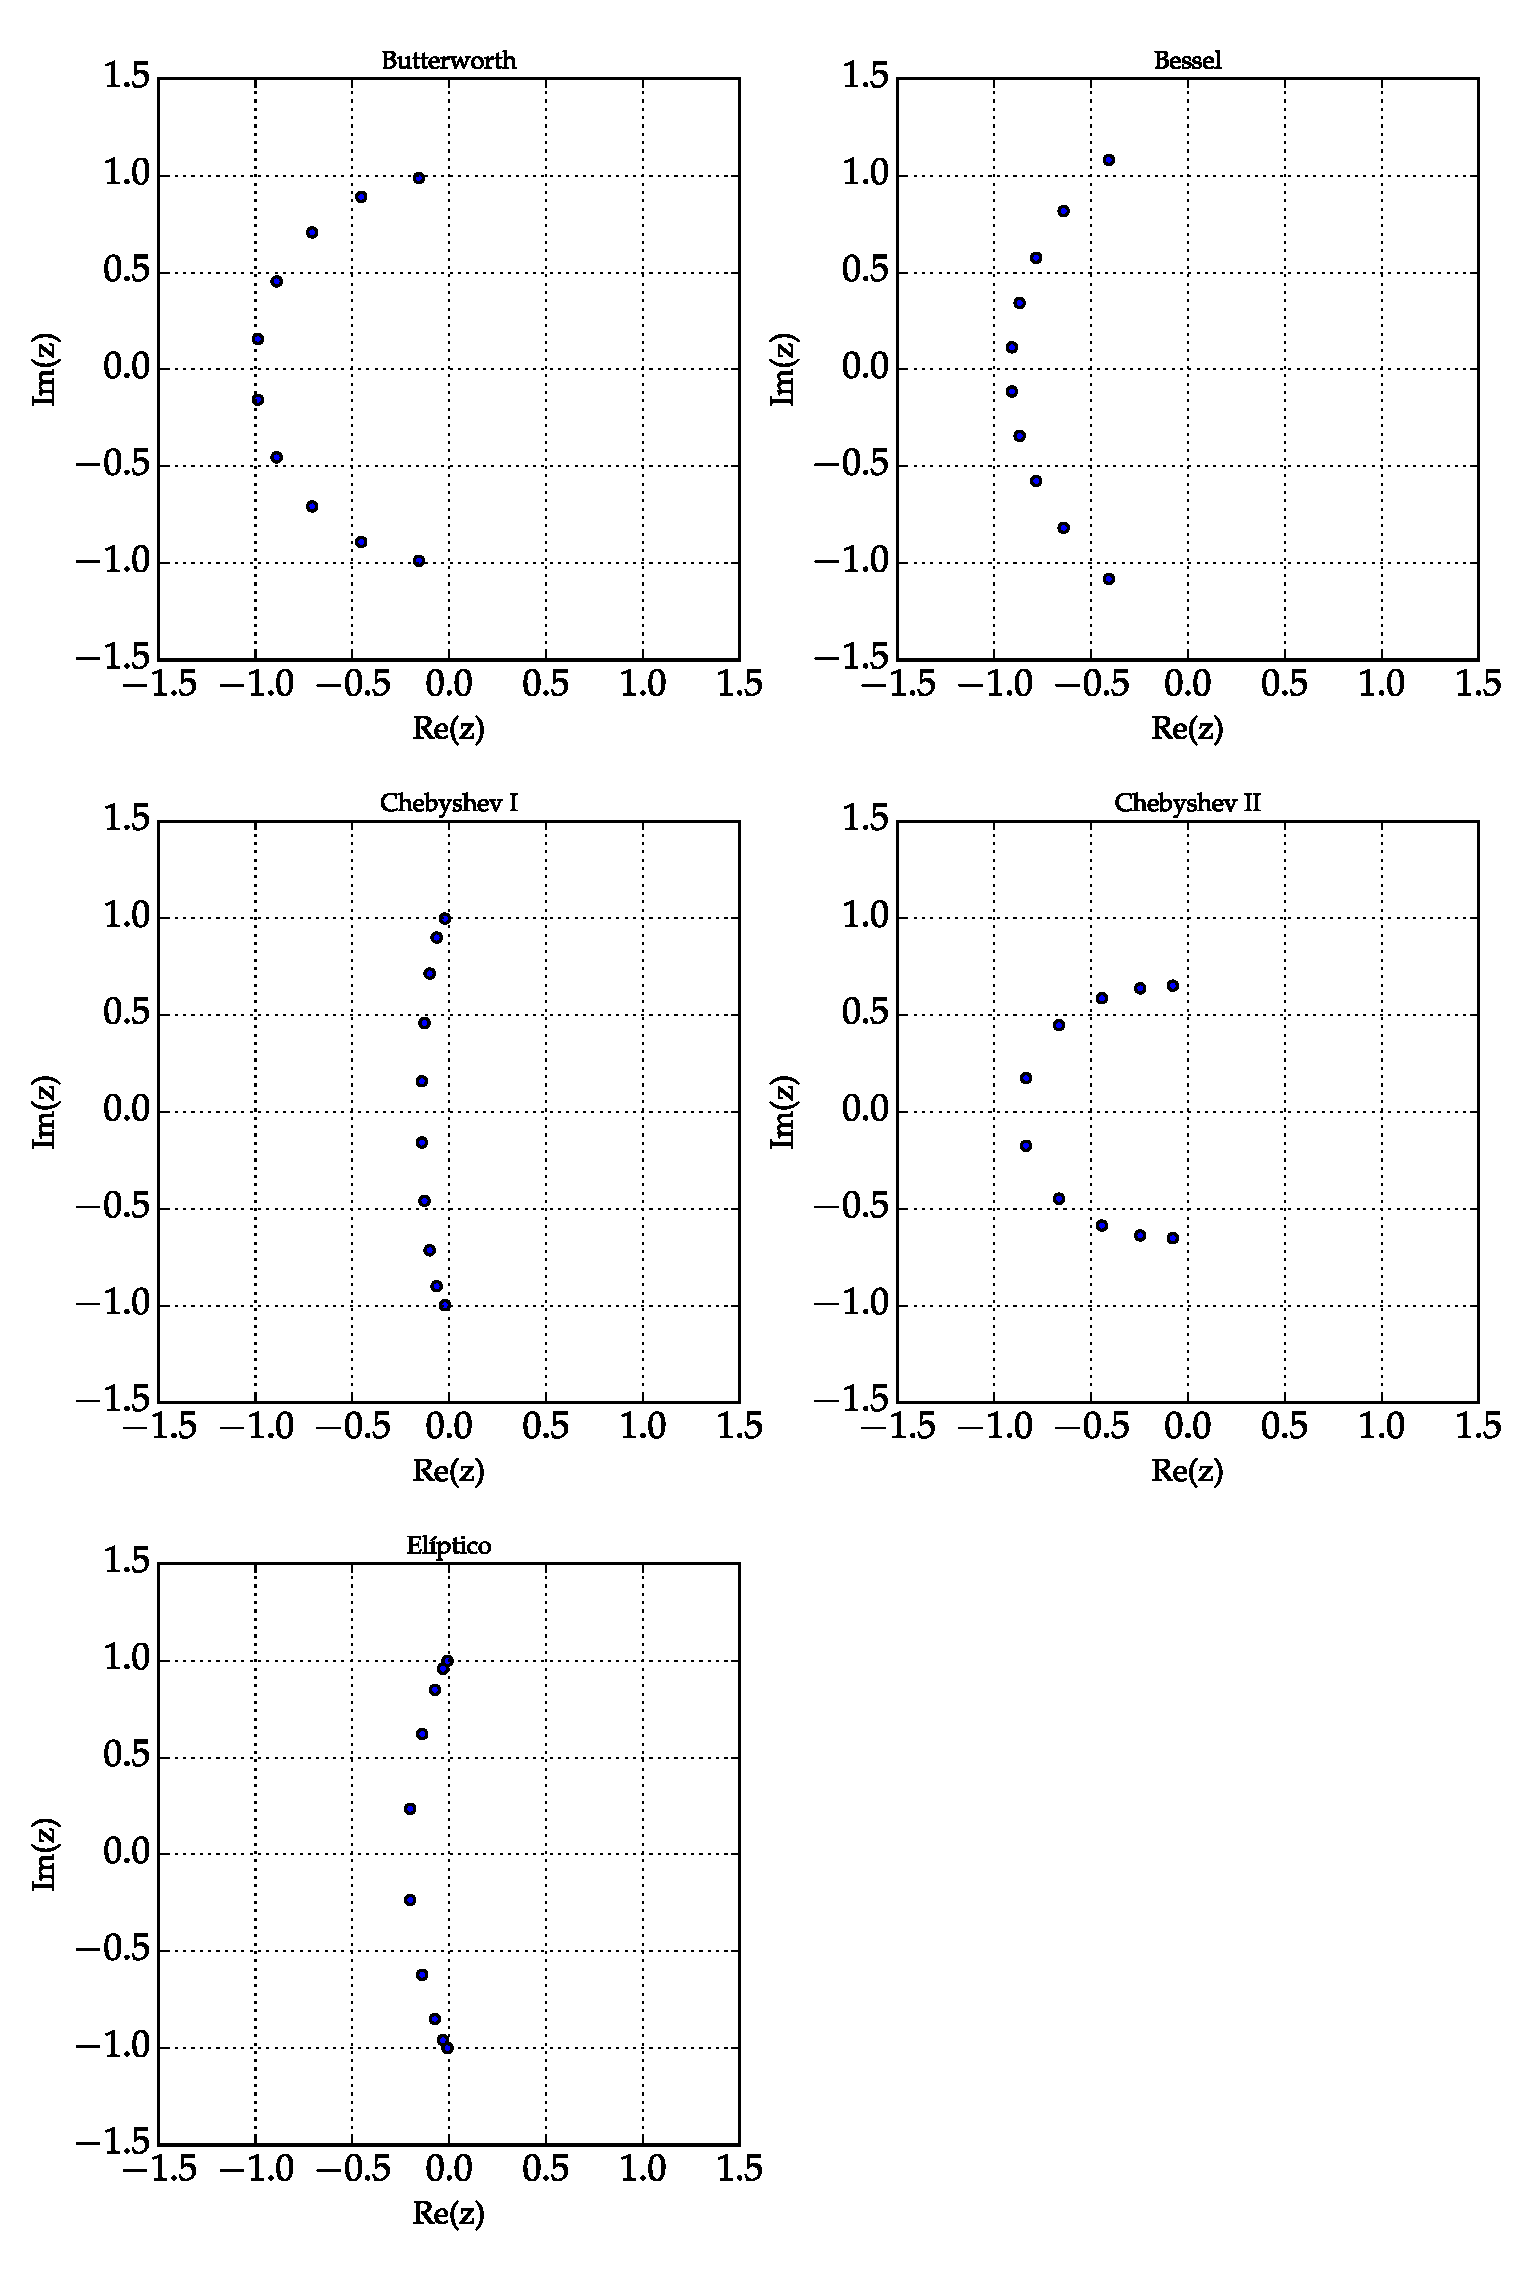
\includegraphics[scale=0.625]{images/plots/filter_comparison}
\caption{Diagramas de polos dos tipos de filtros descritos no capitulo. Todos os filtros têm ordem $N = 10$ e $\omega_c$ = 1 rad/s.}
\label{fig:compare_poles}
\end{figure}

\subsection{Transformação de Filtros}
As funções de transferência acima descritas referem-se ao filtro passa-baixa. Para a obtenção das funções de transferência referentes a outros filtros a partir desta, podem-se realizar as transformações a seguir \cite{zumbalen}:
\begin{itemize}
\item{\textbf{Passa-baixa para passa-alta}:} Multiplicar o numerador por $s^n$, onde $n$ é a ordem do filtro.
\item{\textbf{Passa-baixa para passa-faixa}:} O numerador torna-se $H_0 \omega_0^2 s^n$, onde $n$ é a ordem do filtro e $H_0$ é o ganho do circuito, definido pela expressão $\frac{H}{Q}$ para um valor de $H$ especificado. 

$Q$, por sua vez, é a seletividade do filtro e é calculada por $\frac{F_0}{F_H - F_L}$, na qual $F_0$ é a frequência de ressonância do filtro e $F_H$ e $F_L$ são as frequências onde as respostas são de $3$ e $-3$ dB, em relação ao pico $F_0$, respectivamente. Pode-se demonstrar que $F_0 = \sqrt{F_H F_L}$.

\item{\textbf{Passa-baixa para rejeita-faixa}:} Troca-se $s$ por $\frac{s (\omega_H - \omega_L)}{s^2 + \omega_H \omega_L}$ onde $\omega_H$ e $\omega_L$ são as frequências onde as respostas são de $3$ e $-3$ dB respectivamente.
\end{itemize}


\subsection{Implementação de Filtros}

Obtida a função de transferência, é necessário implementá-la na forma de um circuito eletrônico ativo ou passivo\footnote{Filtros passivos não serão descritos neste trabalho, porém, a implementação deles pode ser feita de forma similar: determina-se um circuito que satisfaça a função de transferência desejada e então decidem-se os valores dos componentes.}.  

Várias topologias são comumente utilizadas, implementando blocos de primeira ou segunda ordem que podem ser cascateados - respeitando-se as impedâncias de entrada e saída e adicionando \textit{buffers} - conforme necessário.

Além de circuitos compostos por resistores e capacitores e que não serão abordados aqui pois sua análise é bastante simples, as topologias mais comuns para filtros ativos são:

\vspace{4cm}

\subsubsection{Topologia \textit{Sallen-Key}}

\begin{figure}[H]
  \centering
  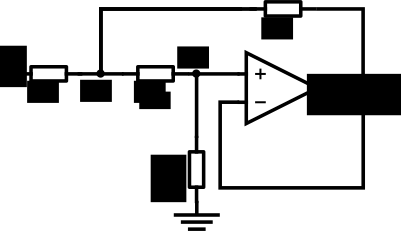
\includegraphics{images/Sallen_Key_generic}
  \caption{Circuito Sallen-Key genérico.}
  \label{fig:sallen_key_generic}
\end{figure}

A partir da figura \ref{fig:sallen_key_generic} podemos realizar a dedução da função de transferência da topologia Sallen-Key para elementos $Z_n$ genéricos e assumido um \textit{op-amp} ideal. Como o amplificador operacional está configurado com realimentação negativa,

\begin{equation}
v_+ = v_- = v_{out}
\label{eq:opamp_negative_oa}
\end{equation}

Aplicando-se a lei dos nós de Kirchoff no nó $V_{x}$ tem-se que 

\begin{equation}
\frac{V_{in} - V_{x}}{Z_1} = \frac{V_x - V_{out}}{Z_3} = \frac{V_x - V_+}{Z_2}
\end{equation}

que pode ser reescrita, usando-se a relação descrita em \ref{eq:opamp_negative_oa}, como

\begin{equation}
\frac{V_{in} - V_{x}}{Z_1} = \frac{V_x - V_{out}}{Z_3} - \frac{V_x - V_{out}}{Z_2}
\end{equation}

Similarmente, fazendo-se a lei dos nós de Kirchoff na entrada não-inversora $V_+$ tem-se que

\begin{equation}
\frac{V_x - V_{out}}{Z_2} = \frac{V_{out}}{Z_4} \rightarrow V_x = V_{out} (\frac{Z_2}{Z_4}+1)
\end{equation}

Combinando-se as expressões para $V_{in}$ e $V_{out}$, pode-se demonstrar que elas representam uma função de transferência da forma 

\begin{equation}
\frac{v_{out}}{v_{in}} = \frac{Z_3 Z_4}{Z_1 Z_2 + Z_3 (Z_1 + Z_2) + Z_3 Z_4}
\label{eq:sallen_key_generic}
\end{equation}

que com os valores adequados dos componentes, representa uma função típica de um sistema de segunda ordem. Por exemplo, definindo-se $Z_1$ e $Z_2$ como resistores de valor $R_1$ e $R_2$ respectivamente, e $Z_3$ e $Z_4$ como capacitores de valores $C_1$ e $C_2$, a função de transferência terá a forma daquela de um filtro passa-baixa, ou seja,

\begin{equation}
H(s) = \frac{1}{R_1 R_2 C_1 C_2 s^2 + C_2 (R_1 + R_2)s + 1}
\end{equation}

O mesmo raciocínio pode ser aplicado para a obtenção das outras funções de transferência a partir da função genérica apresentada em \ref{eq:sallen_key_generic} (por exemplo, trocando-se a posição dos resistores e capacitores, será obtido um filtro passa-alta). Uma análise detalhada desta topologia é feita pelos seus criadores em \cite{sallen}.

\subsubsection{Topologia \textit{Multiple Feedback}}
\begin{figure}[H]
  \centering
  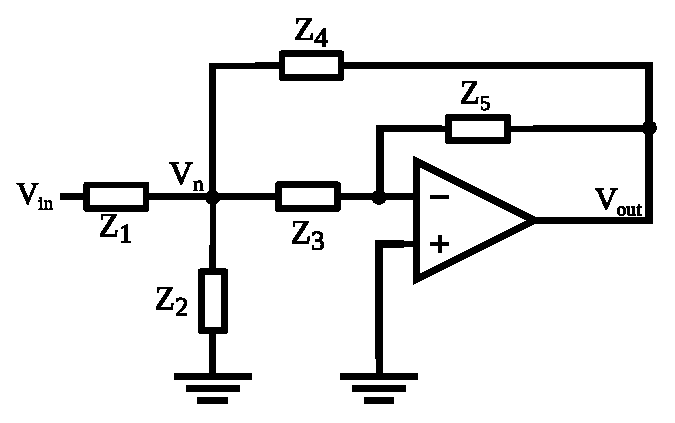
\includegraphics{images/mfb_generic}
  \caption{Circuito \textit{multiple feedback} genérico.}
  \label{fig:mfb_generic}
\end{figure}

Para simplificar a análise do circuito apresentado na figura \ref{fig:mfb_generic}, serão usadas as admitâncias dos componentes, de forma que $Y_n = \dfrac{1}{Z_n}$. Dessa forma, pela lei dos nós de Kirchoff, teremos que, onde $I_n$ refere-se à corrente que passa pelo componente $n$:

\begin{equation}
I_1 = Y_1 (V_{in} - V_{n}) = I_2 + I_3 + I_4 \rightarrow Y_1 V_{in} = V_n (Y_1 + Y_2 + Y_3 + Y_4) - Y_4 V_{out}
\end{equation}

e também que

\begin{equation}
Y_3 V_n = -Y_5 V_{out} \rightarrow V_{n} = -\frac{Y_5 V_o}{Y_3} 
\end{equation}

\begin{equation} 
Y_1 Y_3 V_{in} = V_{out}[-Y_5 (Y_1 + Y_2 + Y_3 + Y_4) - Y_3 Y_4]
\end{equation}

e assim pode-se demonstrar que

\begin{equation}
\frac{H(s)} = \frac{-Y_1 Y_3}{Y_5 (Y_1 + Y_2 + Y_3 + Y_4) + Y_3 Y_4}
\end{equation}.

na qual fazendo-se $Y_1$, $Y_3$ e $Y_4$ resistores e $Y_2$ e $Y_5$ capacitores obtém-se uma função de transferência de um filtro passa-baixa, por exemplo. 

\subsubsection{Topologia \textit{KHN (Kerwin-Huelsman-Newcomb)}}
A topologia KHN (Kerwin-Huelsman-Newcomb), ou de variáveis de estado, é dada pelo circuito:

\begin{figure}[H]
  \centering
  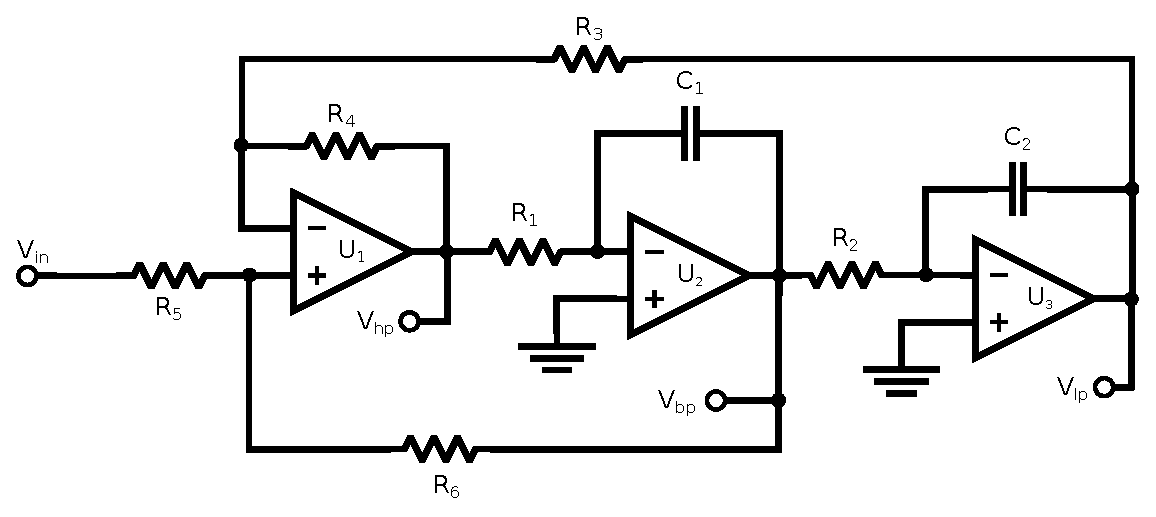
\includegraphics[scale=0.82]{images/khn_generic}
  \caption{Circuito KHN}
  \label{fig:khn_generic}
\end{figure}

Pode-se demonstrar que a função de transferência é, para a saída passa-baixa $V_{lp}$,

\begin{equation}
H_{lp}(s) = \frac{K_{lp} a_0}{s^2 + a_1 s + a_0}
\end{equation}

onde $a_0 = \frac{R_4}{R_3} \frac{1}{R_1 C_1} \frac{1}{R_2 C_2}$, $a_1 = \frac{1+\frac{R_4}{R_3}}{1+\frac{R_6}{R_5}} \frac{1}{R_1 C_1}$ e $K_{lp} = \frac{1+R_3/R_4}{1+R_5/R_6}$ \cite{rowell}.

Similarmente, tomando-se a saída passa-alta $V_{hp}$ na saída do somador $U_1$, determina-se que a função de transferência dela é 

\begin{equation}
H_{hp}(s) = \frac{K_{hp} s^2}{s^2 + a_1 s + a_0}
\end{equation}

com $K_{hp} = \frac{1+R_4/R_3}{1+R_5/R_6}$. $a_0$ e $a_1$ são os mesmos enumerados acima.

E para o filtro passa-faixa, tomado a partir da saída do integrador $U_2$ temos a expressão,

\begin{equation}
H_{bp}(s) = \frac{K_{bp} a_1 s}{s^2 + a_1 s + a_0}
\end{equation}

onde $K_{bp} = \frac{R_6}{R_5}$.

Somando-se as saídas do filtro passa-baixa e passa-alta, pode-se construir o filtro rejeita-faixa.

\subsubsection{Vantagens e Desvantagens de Cada Topologia}
As topologias \textit{Sallen-Key} e \textit{Multiple Feedback} são bastante simples e exigem poucos componentes, o que reduz o seu consumo de energia e proporciona uma implementação mais fácil; todavia, elas são mais sensíveis às variações dos dispositivos empregados \cite{an738} \cite{an1762}. 

Já a topologia KHN exige três op-amps que deverão ter uma largura de banda maior devido a estarem configurados como integradores (alguns autores, ex. \cite{jung}, recomendam uma largura de banda 10 vezes maior que a frequência de corte do filtro); todavia, eles apresentam menor sensitividade, pois as variações dos componentes (assumindo que eles sejam relativamente similares) tenderão a se cancelar; além disso, esta topologia é insensível a variações no ganho dos amplificadores operacionais (uma análise de sensibilidade é feita detalhadamente em \cite{khn}).

Além disso, ela permite obter os três tipos de filtro mais comuns (passa-baixa, passa-alta e passa-faixa) a partir do mesmo circuito - e, com uma pequena modificação, obtém-se o filtro rejeita-faixa. 

Visto que a topologia KHN é bastante comum, alguns fabricantes fornecem circuitos integrados (por exemplo, UAF42 da Texas Instruments \cite{uaf42}) com três \textit{op-amps} no mesmo componente, bastando então adicionar os resistores e capacitores para as frequências desejadas.

Dessa forma, a seleção da topologia a ser empregada envolve um \textit{trade-off} entre custo, consumo de energia, sensibilidade às variações dos componentes e complexidade de projeto.

\section{Filtros Digitais}

\subsection{Famílias de Filtros Digitais}
Existem duas famílias de filtros digitais: os filtros FIR (\textit{Finite Impulse Response}) e IIR (\textit{Infinite Impulse Response}). Como seus próprios nomes dizem, o fator que diferencia essas duas categorias é a resposta ao impulso (isto é, a um sinal $x$ no qual $x_0$ = 1 e $x_n = 0$ para todo $n \geq 1$).

\subsubsection{Filtros FIR (\textit{Finite Impulse Response})}

Esta família de filtros, para um filtro de ordem $N$, pode ser descrita por uma equação da forma

\begin{equation}
y_n = b_0 x_n + b_1 x_{n-1} + \dots + b_N x_{n-N} \equiv \sum_{i=0}^{N} b_i x_{n-i}
\label{eq:fir_sum}
\end{equation}

onde:

\begin{itemize}
\item $x$ é o sinal de entrada;
\item $y$ é o sinal de saída;
\item $N$ é a ordem do filtro;
\item $b_i$ são os coeficientes do filtro.
\end{itemize}

Sendo constituída apenas por zeros e não tendo polos, essa família de filtros não têm problemas de estabilidade. 

\subsubsection{Filtros IIR (\textit{Infinite Impulse Response})}
Esta família de filtros é projetada, em geral, a partir das funções de transferência dos filtros analógicos, realizando-se a transformação para o tempo discreto empregando-se, por exemplo, a transformada de Tustin que será descrita a seguir.

Ela em geral é implementável com menos cálculos, porém, requer cuidados com a sua estabilidade por possuir \textit{feedback}. 

\subsection{Algoritmos para Projeto de Filtros Digitais}

\subsubsection{Projeto de filtros FIR: método da janela}

Inicialmente, determina-se um filtro ideal que atenda à função de transferência desejada. Isso pode ser feito realizando-se a transformada discreta inversa de Fourier: em geral, o filtro obtido (chamado de $h_{ideal}$) será não-causal e, conforme já explicado na seção \ref{sec:analog_filters}, escrito em termos da função sinc \cite{haykin}. 

Para tornar esse filtro causal, poderíamos simplesmente truncá-lo na ordem desejada, porém, isso resulta no fenômeno de Gibbs visível na figura \ref{fig:gibbs}, comportamento fortemente oscilatório nas descontinuidades \cite{haykin}:

\begin{figure}[H]
  \centering
  \includegraphics[scale=0.5]{images/plots/gibbs}
  \caption{O fenômeno de Gibbs para uma soma de senoides.}
  \label{fig:gibbs}
\end{figure}


Dessa forma, o filtro é transformado em causal empregando-se uma função janela (\textit{window function}). Funções janela são funções cuja definição, para um filtro de ordem $N$, é dada por

\[ w[n] = \begin{cases} 
      f[n, N] & 0 \leq n \leq N \\
      0 & \text{outros casos} \\
   \end{cases}
\]

Existem diversas funções janela descritas na literatura (por exemplo, \cite{diniz} descreve cerca de 10 delas e \cite{harris} descreve cerca de 20 mais utilizadas), sendo que as mais comuns são:

\begin{itemize}
\item retangular (isto é, $w[n] = 1$ para todo $n \leq N$);
\item de Hamming, dada por

\[ w[n] = \begin{cases} 
      0.54 - 0.46 \cos{\frac{2 \pi n}{N}} & 0 \leq n \leq N \\
      0 & \text{outros casos} \\
   \end{cases}
\]
\item triangular, dada por 

\begin{equation}
w[n] = 1 - \left|\frac{n-\frac{N-1}{2}}{\frac{N}{2}}\right|
\end{equation}

\end{itemize}

Feito isso, obtém-se o novo filtro $h[n]$ por meio da convolução $h_{ideal}[n] \times w[n]$. Esse filtro será causal, linear e invariante no tempo.

Não existe um critério para a seleção da função janela a ser empregada no projeto; em \cite{harris}, são propostas algumas figuras de mérito para comparar estas funções (por exemplo, a amplitude dos lóbulos laterais (\textit{side lobes}) e a largura do lóbulo principal, como visto na figura \ref{fig:window_functions}), porém a decisão será do projetista que deverá considerar todos os fatores envolvidos para o projeto do filtro (\textit{ripple} aceitável, atenuação desejada, velocidade da transição da banda de passagem para a banda de parada etc...).

\begin{figure}[H]
  \centering
  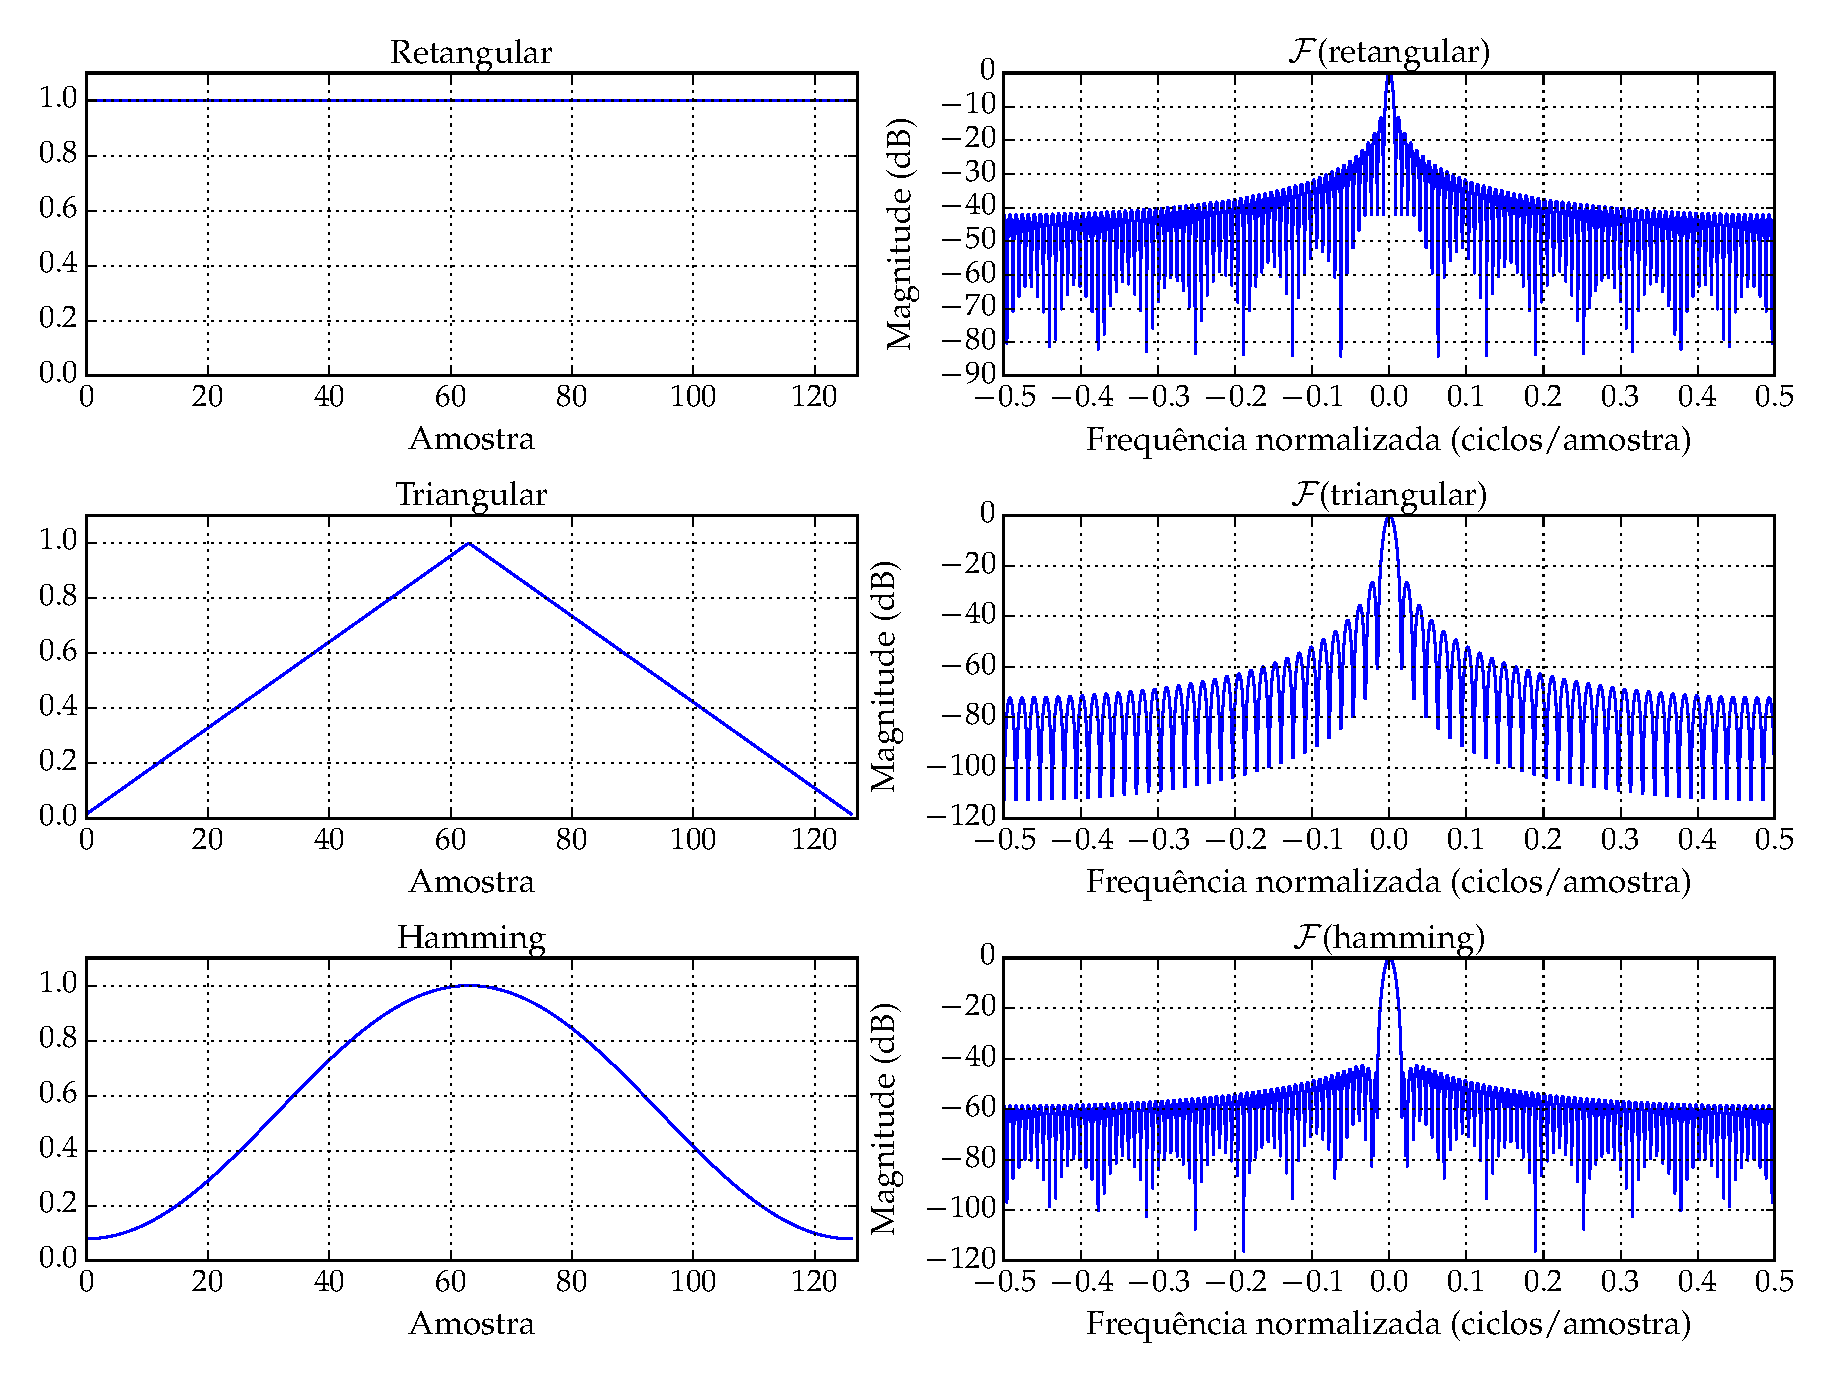
\includegraphics[scale=0.5]{images/plots/window_functions}
  \caption{Funções janela mais comuns e sua transformada de Fourier.}
  \label{fig:window_functions}
\end{figure}


\subsubsection{Projeto de filtros FIR: algoritmo de Parks-McClellan}
O método da janela, embora simples para filtros de pequena ordem e capaz de fornecer resultados \textit{bons o suficiente} para muitas aplicações, torna-se pouco prático e já não fornece resultados ótimos à medida que a ordem cresce ou para filtros mais complexos (por exemplo, filtros que permitam a passagem de múltiplas faixas de frequências). 

A estratégia adotada por \cite{mcclellan}, então, é tratar o projeto de filtros como um problema de otimização, isto é, encontrar coeficientes que aproximem a forma desejada para a resposta em frequência, ao mesmo tempo em que se minimiza o \textit{ripple} desta aproximação. Esse algoritmo será explicado mais detalhadamente no capítulo relativo ao desenvolvimento da ferramenta.

\subsubsection{Projeto de filtros IIR: Conversão de um Filtro Analógico em Digital}
Para o projeto de filtros IIR, é comum projetar um filtro analógico equivalente e depois convertê-lo para um filtro digital, escrevendo-se sua função de transferência $H(z)$ a partir da função de transferência $H(s)$ do filtro analógico projetado.

Existem diversos métodos para tal; o método mais comum e implementado nesse trabalho é o método de Tustin ou transformada bilinear \cite{haykin}. Para este método, seja $z = e^{s T}$. Reescrevendo-se essa função em termos de $s$, ter-se-á que $s = \frac{\ln(z)}{t}$.

A série de Taylor em função de $z$, truncada para o primeiro termo (suficiente para nossa aplicação) é 

\begin{equation}
s \approx \dfrac{2}{t} \dfrac{z-1}{z+1}
\label{eq:tustin_formula}
\end{equation}

onde $t$ é o tempo de amostragem ($t = 1/f_s$). Um fenômeno que acontece nesta de conversão é o \textit{warping} das frequências, o qual encontra-se descrito mais detalhadamente, por exemplo, em \cite{haykin}.

%Seja a equação \ref{eq:tustin_formula} reescrita em função de $s$, isto é, para $t = 2$:

%\begin{equation}
%z = \frac{1+s}{1-s}
%\end{equation}. 

%Então, defina-se $s = \sigma + j\omega$ e $z = re^{i \theta}$. Dessa forma, determina-se que $r = |z| = \sqrt{\frac{(1+\sigma)^2 + \omega^2}{(1-\sigma)^2 + \omega^2}}$ e que $\theta = \arctan{\frac{\omega}{1+\sigma}} + \arctan{\frac{\omega}{1-\sigma}}$. Assumindo-se $\sigma = 0$ (pois estamos no regime permanente) pode-se deduzir que  \cite{haykin}

%\begin{equation}
%\omega = \tan{\frac{\Omega}{2}}
%\label{eq:tustin_warp}
%\end{equation}
%\end{comment}

Para que o filtro projetado tenha a devida frequência de corte, realiza-se o procedimento conhecido como \textit{prewarp}: sendo $\Omega$ a frequência de $-3$ dB desejada no filtro digital, determina-se o $\omega$ para projeto de um filtro analógico equivalente empregando-se a expressão $\omega = \tan{\frac{\Omega}{2}}$ \cite{haykin}.

\subsection{Comparação: Filtros FIR e IIR}
A vantagem imediata dos filtros FIR é sua estabilidade incondicional, por não possuírem \textit{feedback}. Entretanto, eles requerem um maior número de cálculos (e, portanto, mais tempo de processamento e mais memória, além de causarem um \textit{delay} na saída) para chegar no mesmo resultado que pode ser obtido com um filtro IIR.

Porém, o projeto dos filtros IIR requer menos passos e a sua implementação, em geral, possui melhor desempenho por exigir menos armazenamento em memória e menos cálculos que os filtros FIR. Torna-se mais fácil obter um filtro IIR que atinja uma especificação desejada, pois pode-se partir do conhecimento de filtros analógicos e, após, discretizar o filtro projetado.

\section{Comparação: Filtros Digitais e Analógicos}
Ainda que o custo das CPUs esteja caindo ao mesmo tempo em que seu desempenho aumenta, os filtros analógicos têm como principal vantagem o seu baixo custo para pequenas ordens: são necessários resistores, capacitores e amplificadores operacionais, ao passo que filtros digitais demandam uma CPU com o desempenho necessário para a aplicação e o desenvolvimento de algoritmos - uma atividade que, por si só, pode ser mais demorada e dispendiosa que o projeto de um circuito. 

Filtros analógicos também são obrigatórios para os circuitos de \textit{antialiasing} de conversores A/D e D/A, ou para operação em frequências muito altas ou baixas. Porém, eles sofrem com a variabilidade dos componentes empregados para sua construção - componentes mais precisos também são mais caros; este problema não ocorre em um filtro digital no qual coeficientes e valores são armazenados na memória da CPU e se mantém estáveis.

Nos filtros digitais, a ordem máxima é limitada principalmente pelo desempenho da CPU utilizada e pelas características dos conversores de dados empregados: conforme afirmado anteriormente, a CPU tem um intervalo de tempo inversamente proporcional à frequência de amostragem para realizar os cálculos. Assim, a aplicação dos filtros digitais em altas frequências torna-se complexa e limitada - embora, com o tempo e a evolução do \textit{hardware}, isso tenda a se tornar um problema cada vez menor.

Conclui-se, então, que os filtros analógicos são desejáveis em aplicações onde o custo e simplicidade são críticos e/ou frequências altas (a partir de de algumas centenas de KHz) ou muito baixas (na faixa de alguns poucos Hz) estão envolvidas; já os filtros digitais apresentam como importante aspecto a sua flexibilidade e a possibilidade da implementação de filtros com ordens maiores.